\documentclass[professionalfonts, xcolor={usenames,svgnames,x11names,table}]{beamer}

\usetheme{SBUclass}
\usepackage[charter]{mathdesign}
\usepackage[scaled]{helvet}

\usepackage{mypackages}

\title{\texorpdfstring{Fundamentals of Python}{Fundamentals of Python}}
\subtitle{Syllabus}
\author{Aniello De Santo}
\institute{University of Utah\\\texttt{aniello.desanto@utah.edu}}
\date{Aug 26, 2020}


\begin{document}
\unnumbered{
\begin{frame}
	\titlepage
\end{frame}
}

\begin{frame}{Organizational Information}
    \begin{center}
        \begin{tabular}{r@{\hspace{2em}}l}
            \textbf{Course}            & Fundamentals of Python\\
            \textbf{Course\#}          & LING 5981/6080\\
            \textbf{Room}              & GC 2575 \\
           \textbf{Time - Mondays}             & Asynchronous\\ 
              \textbf{Time  - Wednesdays}              & W 3:00--4:20\\ 
            \textbf{Website}           & Canvas and Slack \\[12pt]
            \textbf{Instructor}        &  Aniello De Santo\\
            \textbf{Pronouns}        &  he/his/him\\
            \textbf{Email}   &       \url{aniello.desanto@utah.edu}  \\
             \textbf{Office hours}      & M 1:30 -- 3:00 ; W 2:00 -- 3:50\\
	\textbf{Online only meeting}      &  W 1:30 -- 2:00\\
            \textbf{Office}            & Zoom\\[12pt] 
        \end{tabular}
    \end{center}
    See the Canvas course page for more details and announcements.
\end{frame}


\begin{frame}{Catalog Description}
    \small

 This course is an introduction to programming principles using Python.
Students will acquire basic programming skills, knowledge of fundamental coding concepts, and the ability to write scripts for simple language-oriented tasks.
Linguistic examples will be used to motivate the introduction of new coding concepts.
We will discuss the language technologies of our daily life - spam filtering, machine translation, and more - and how they work under the hood.  

No previous training in mathematics, linguistics, or computer science required.

\end{frame}



\begin{frame}{Learning How to Code?}
    By the end of the course, you will have basic Python literacy.\\
  More importantly, you should have refined your problem solving skills.
    %
    \begin{center} 
         \href{https://www.youtube.com/watch?v=k5iEc6TP_50}{
            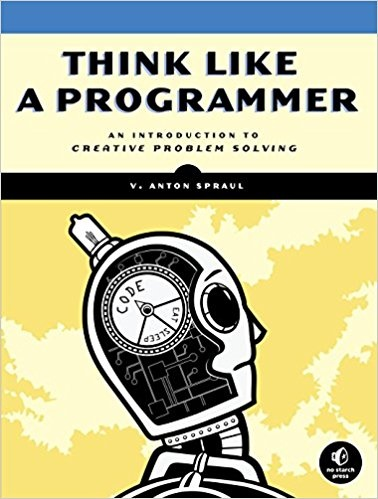
\includegraphics[width=.45\linewidth]{img/think}}
    \end{center}
\end{frame}

\begin{frame}{An Experiment}
    \begin{enumerate}
        \item Open some chat or messaging app on your phone.
        \item Start typing a random letter.
        \item Click the second word suggestion\\
              (the one in the middle).
        \item Keep doing the previous step for a while (say, 10 to 15 words).
        \item Did you get a reasonable sentence of English?
    \end{enumerate}

    \visible<2>{
        \begin{quote}
            I am a beautiful person who is the best of luck to you by the way to get the best of luck to you by the way to get the best of luck to you by the way to get the \ldots
        \end{quote}
        }
\end{frame}

\begin{frame}{An Experiment (part 2)}
    \begin{center}
        \begin{tikzpicture}
            \node[draw=Blue3,fill=Blue3!25,thick,
                  font=\LARGE\bfseries, align=center,
                  inner sep=1em] at (0,0) %
                {Give me instructions \\on how to open my water bottle};
        \end{tikzpicture}
    \end{center}
\end{frame}

\begin{frame}{Goals and Objectives}
    \begin{itemize}
	\item  acquire core programming skills generalizable to any programming language
	\item master essential concepts and techniques in Python programming
	\item translate abstract computational models into fully functional source code
	\item develop learning autonomy and the ability to deepen your programming knowledge through self-study
    \end{itemize}
\end{frame}


\begin{frame}{Prerequisites}
    \begin{itemize}
        \item \textbf{What You Need}
            \begin{itemize}
                \item ability to operate a computer\\
                    (use a web browser, install software, edit text files)
                \item willingness to play around with open-ended problems
            \end{itemize}
        %
        \item \textbf{What You \highlight{WON'T} Need}
            \begin{itemize}
                \item programming experience
                \item math (except for addition, multiplication and fractions)
                \item linguistics
            \end{itemize}
    \end{itemize}
\end{frame}

\begin{frame}{Course Set Up}

\begin{itemize}
   \item \textbf{Lecture notes and HW} written in Jupyter Notebook
   \item I suggest using Google CoLab for execution
   \item \textbf{Participation and peer discussion} Course Slack channel \\ (get in touch if your invite has expired)
       \end{itemize}
\end{frame}

\begin{frame}{Two Types of Instruction}
    \begin{description}
        \item[Monday] Asynchronous guided self study\\
        				Notebooks with study materials uploaded on Canvas
        \item[Wednesday] in-class programming sessions in Python\\
        					\textbf{come with questions!}
    \end{description}

    \begin{block}{Online only students...}
... will meet with me once per week for regular check ins. 
    \end{block}

    \pause
    \begin{block}{What happens if we all move online?}
 In case of a sudden move to full online instruction, Wednesday lectures will become discussion sessions via Zoom. Each student will be required to submit a question beforehand. 
    \end{block}
\end{frame}

\begin{frame}{Grading Components}
    \textbf{Class Participation (25\%)}
        \begin{itemize}
            \item Both in class and \highlight{online}!
            \item \textbf{Examples}:
                \begin{itemize}
                    \item ask questions (in person, via email, via Slack)
                    \item help fellow students (in person, via Slack)
                    \item link to relevant online materials (e.g. in Slack)\\
                        $\vdots$
                \end{itemize}
            \item \textbf{Why?} 
                \begin{itemize}
                    \item Encourages you to ask questions.
                    \item Helping others is a great way of learning.
                    \item We want to have some fun, too.
                \end{itemize}
        \end{itemize}
\end{frame}

\begin{frame}{Grading Components [cont.]}
    \textbf{Python Exercises (70\%)}
        \begin{itemize}
            \item once per week
            \item programming in \highlight{Python}
            \item assigned on Mondays 
            \item due the following Sunday at 11:59pm
            \item assigned via  Canvas, collected via email
            \item late hand-ins?
            \item \textbf{Why?}
                \begin{itemize}
                    \item Learning programming is like learning a new language\\
                            $\Rightarrow$ needs constant practice
                    \item Even a little bit of programming experience is incredibly useful.
                \end{itemize}
        \end{itemize}
\end{frame}


\begin{frame}{Grading Components [cont.]}
  \textbf{Midterm (5\%)}
 \begin{itemize}
            \item Tentatively in \highlight{Week 9} 
            \item Pen-and-paper coding assignment        
              \item \textbf{Why?}
                \begin{itemize}
                    \item Force you to check how your study method is working, and eventually correct course
                    \item Pen-and-Paper coding helps focus on solving the problem and not on the minor details of the coding language (i.e. Python).
                \end{itemize}    
            \end{itemize}
            \textbf{Dealing with Fails}
                \begin{itemize}
                                  \item Extra-credit opportunities (5\% each)
                     			     \begin{itemize}
          			  \item Participate to department events
                            \item Participate to online experiments (info on Canvas)
                                \end{itemize}
        \item Optional  \highlight{Final project} for Python.
        			     \begin{itemize}
            		             \item Extra-credit, worth up to 10\% of the total grade
                                       \item Due during finals week together with a class survey.
                                \end{itemize}
                    \end{itemize}     
\end{frame}

\begin{frame}{Soapbox: Thoughts on Grades}

    \begin{center}
        \begin{tabular}{cccc}
            \visible<0->{
\includegraphics[width=7em]{./img/mugger1}} &
            \visible<0->{
\includegraphics[width=7em]{./img/mugger2}} &
            \visible<0->{
\includegraphics[width=7em]{./img/mugger3}} &
            \visible<0->{
\includegraphics[width=7em]{./img/mugger4}}
        \end{tabular}
\end{center}
\pause
    \begin{itemize}
        \item Students are caught up in the \highlight{grade bubble}:
            \begin{itemize}
                \item If I get good grades I will get a job.
                \item If I get bad grades I will fail in life.
            \end{itemize}
        \item In the real world, nobody cares about your GPA.
        \item Don't focus on grades!
        \item Focus on mastering the skills you need to get the job you want.
    \end{itemize}
\end{frame}

\begin{frame}{Soapbox: Our Role in This}
    \begin{itemize}
        \item Instructors are the academic equivalent of a \highlight{fitness trainer}.
        \item You're paying thousands of dollars for us to get you into shape,\\ and we've developed a program for you that will do that.
        \item But you are the one who has to move their body.
        \item Bad techniques like cram learning may get you a good grade,\\
              but you're cheating yourself out of true progress.
        \item If you aren't working towards long-term intellectual growth,\\
            you're flushing tons of money down the toilet.
    \end{itemize}
\end{frame}

\begin{frame}{The steep learning curve! }

%%        
\begin{columns}
\begin{column}{0.5\textwidth}
%  \textbf{It's a steep learning curve!}
        \begin{itemize}
        \visible<2->{\item Don't despair! It takes time!}
        \end{itemize}
        \vspace{0.5cm}
          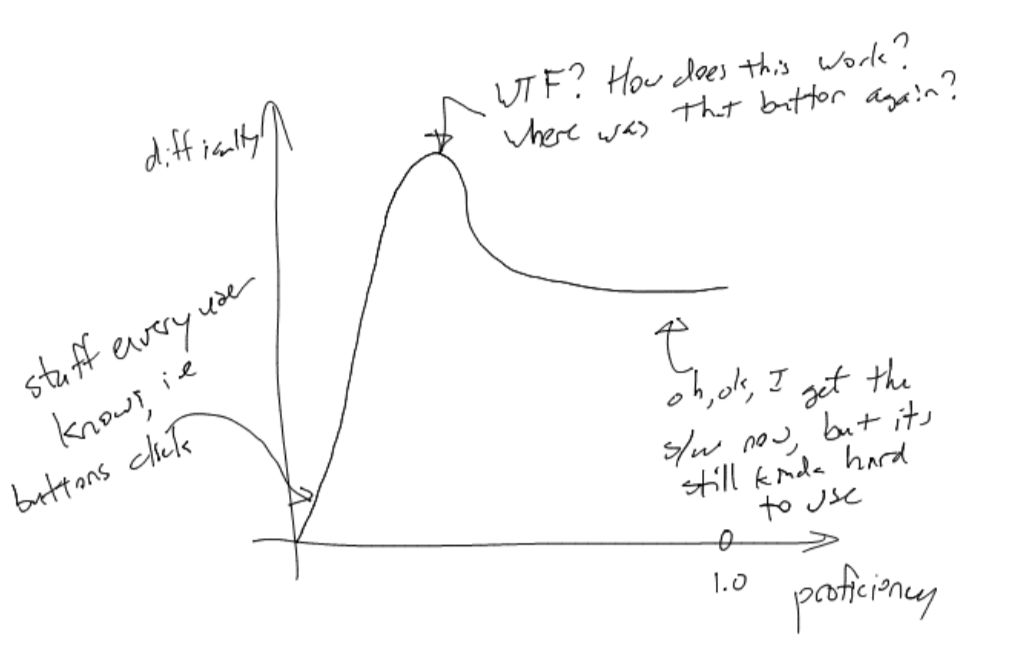
\includegraphics[width=30em]{./img/learning_curve}
\end{column}
\begin{column}{0.5\textwidth}
\visible<2->{
\includegraphics[width=14em]{./img/coding}}
\end{column}
\end{columns}
\end{frame}


\begin{frame}{TL/DR: Ask for Help}
    \begin{itemize}
        \item \textbf{Take advantage of me}\\
            I put a lot of effort into helping you achieve your goals:
            %
            \begin{itemize}
            	\item self-study materials
                \item office hours
                \item availability via email and zoom
            \end{itemize}
            %
            Give me (constructive) feedback on problems with the materials!
            
        \item \textbf{Take advantage of each other}\\
            Your peers are a valuable resource, too.
            Discuss homework, exchange ideas, share notes.
            Collaborate, help each other.

        \item \textbf{Don't wait too long}\\
            The Matthew effect also applies to education: the rich get richer, the poor get poorer.
            If you sense yourself falling behind, ask for help right away.
            The longer you wait, the worse it gets.
    \end{itemize}
\end{frame}

\begin{frame}{Getting Help}
    \begin{itemize}
        \item By default: use Slack
\end{itemize}

 \textbf{Optimizing Response Time}
  \begin{itemize}
        \item Minor technical issue? \\ $\rightarrow$ Slack > Me
         \item Homework/General Python Question?  \\ $\rightarrow$   Slack  > Me
         \item Grading question? $\rightarrow$  Me
         \item Personal Issues?  $\rightarrow$ Me
    \end{itemize}
    \end{frame}
             
 \begin{frame}{Getting Help [cont]}      
   \begin{itemize}      
        \item Contacting me:
            \begin{itemize}
                \item \textit{\{aniello.desanto\}@utah.edu}
                \item Put [LING 5981/6080] at the beginning of the email \textit{Subject}
                \item Reply time usually $<$ 24h (no guarantee during weekends!)
                \item If you plan to come to our office hours but anticipate a long meeting, drop me a line 
                    the day before.
                     \item  If there's a scheduling conflict, I'll let you know.
                    Radio silence means everything is fine.
            \end{itemize}
    \end{itemize}
\end{frame}



%\begin{frame}{Some Final Remarks}
%    \begin{enumerate}
%        \item \textbf{Course Website}
%            \begin{itemize}
%                \item Familiarize yourself with CoCalc and Blackboard.
%                \item Lots of extra information there.
%                        \item Check your SBU email frequently for Blackboard Announcements!
%            \end{itemize}
%        \item \textbf{Software Setup}
%            \begin{itemize}
%                \item We will be using mostly \highlight{CoCalc}.
%                \item You will be invited to join today (via your SBU email).
%                \item You have to pay a 14 dollars subscription within the first two weeks, to ensure:
%                      \begin{itemize}
%                      \item a fast CoCalc Virtual Machine
%                      \item usable with internet connection
%                      \end{itemize}
%                \item More information in Wednesday lecture and in the Friday recitation.
%                \item Get in touch if you have problems!
%            \end{itemize}
%    \end{enumerate}
%\end{frame}

\begin{frame}{Supplementary Textbook (Optional!)}
    \begin{columns}
        \column{.65\linewidth}
            \begin{itemize}
                \item Al Sweigart (2015):\\
                      \emph{Automate the Boring Stuff with Python}
                \item online version \highlight{free}
                \item digital versions and hardcopy around \$25
                \item supplementary \href{https://www.youtube.com/playlist?list=PLGoJzB271_7r-iLYuEHEPJ5pSIYxXjJEn}{videos on Youtube}
                \item \highlight{It is not required}\\
                      but it's a good source to consult if something is unclear.
            \end{itemize}

        \column{.35\linewidth}
            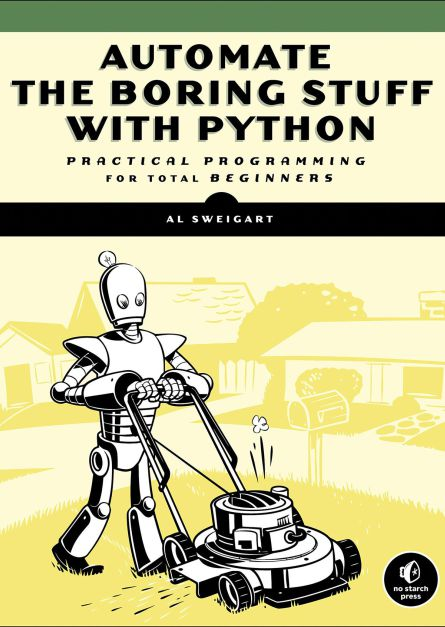
\includegraphics[width=.9\linewidth]{./img/textbook}
    \end{columns}
\end{frame}

\begin{frame}{Tentative Schedule}
\begin{table}[]
\resizebox{\linewidth}{!}{
\begin{tabular}{llll}
\multicolumn{1}{c}{Week} & \multicolumn{1}{c}{Monday}                    & \multicolumn{1}{c}{Wednesday} & \multicolumn{1}{c}{HW \# Due} \\ \hline
1                        & Syllabus                                      & Intro  to Jupyter and Colab   & No HW Due                     \\
2                        & Notebook 1: Variables and Data Types          &                               & No HW Due                     \\
3                        & Labor day                                     & Notebook 2: Flow control      & HW 1 Due                      \\
4                        & Notebook 3: Lists and for-loops               &                               & HW 2 Due                      \\
5                        & Notebook 4: String Methods                    &                               & HW 3 Due                      \\
6                        & Notebook 5: Dictionaries  (fully online)      &                               & HW 4 Due                      \\
7                        & Notebook 6: File IO (fully online)            &                               & No HW Due                     \\
8                        & Notebook 7: While loops                       &                               & HW 5 Due                      \\
9                        & Midterm  Practice and Q\&A                    & Midterm                       & HW 6 Due                      \\
10                       & Notebook 8: Function definition               &                               & No HW Due                     \\
11                       & Notebook 9: REG Expressions                   &                               & HW 7 Due                      \\
12                       & Notebook 10: Classes                          &                               & HW 8 Due                      \\
13                       & Notebook 10: Advanced N-gram                  &                               & HW 9 Due                      \\
14                       & Buffer  (maybe data manipulation with pandoc) &                               & HW 10 Due                     \\
15                       & Buffer   \& General discussion (fully online) &                               & No HW Due                     \\
16                       & Finals week                                   & Class Survey Due              & No HW Due                    
\end{tabular}}
\end{table}
\end{frame}

\begin{frame}{A Recap: Format  from now on}
    \begin{enumerate}
        \item Notebook X will be uploaded Sunday night
        \item Work on it through the week
        \begin{itemize}
        \item Play with the example code
        \item Do the practice exercises
        \item start looking at the HW questions
        \end{itemize}
        \item Come on Wednesday with questions
        \begin{itemize}
        \item We will look together at the main concerns
        \item We will look at the HW exercises
        \item We will do extra practice
        \end{itemize}
        \item Submit the HW via email by Sunday night.
         \end{enumerate}
\end{frame}


%\begin{frame}{Disability Support Services}
    If you have a physical, psychological, medical or learning disability that may impact your course work, please contact Disability Support Services, ECC (Educational Communications Center) Building, Room 128, (631) 632-6748. They will determine with you what accommodations, if any, are necessary and appropriate. All information and documentation is confidential.

    Students who require assistance during emergency evacuation are encouraged to discuss their needs with their professors and Disability Support Services.
    For procedures and information go to the following website:
    \url{http://www.stonybrook.edu/ehs/fire/disabilities}
\end{frame}

\begin{frame}{Academic Integrity}
    Each student must pursue his or her academic goals honestly and be personally accountable for all submitted work. Representing another person's work as your own is always wrong.  Faculty are required to report any suspected instances of academic dishonesty to the Academic Judiciary.  Faculty in the Health Sciences Center (School of Health Technology \& Management, Nursing, Social Welfare, Dental Medicine) and School of Medicine are required to follow their school-specific procedures. For more comprehensive information on academic integrity, including categories of academic dishonesty, please refer to the academic judiciary website at
    \url{http://www.stonybrook.edu/uaa/academicjudiciary/}
\end{frame}

\begin{frame}{Critical Incident Management}
    Stony Brook University expects students to respect the rights, privileges, and property of other people. Faculty are required to report to the Office of Judicial Affairs any disruptive behavior that interrupts their ability to teach, compromises the safety of the learning environment, or inhibits students' ability to learn.  Faculty in the HSC Schools and the School of Medicine are required to follow their school-specific procedures.
\end{frame}

\end{document}
